

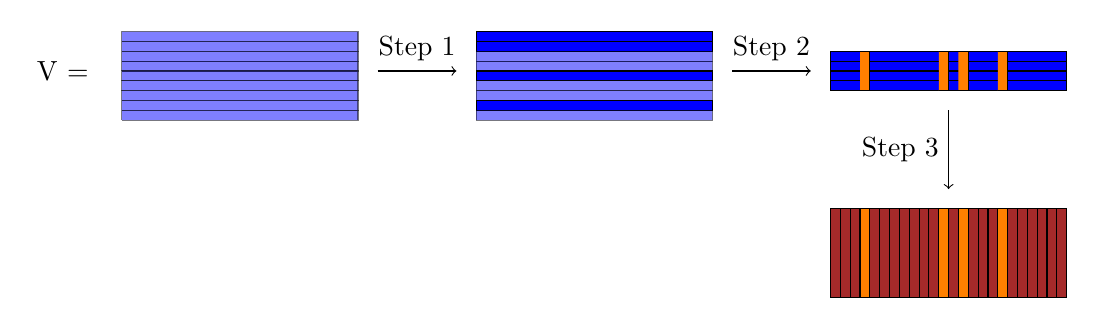
\begin{tikzpicture}[scale = 0.5]

  % draw line and angle
%  \draw
%     pic [draw,angle radius=4mm,angle eccentricity=1.5, "$\theta$" font=\scriptsize] {angle=v2--v1--v3};



\draw [fill=blue, opacity=0.5] (-16,3.75) -- (-10,3.75) -- (-10,4) -- (-16,4) -- (-16,3.75);
\draw [fill=blue, opacity=0.5] (-16,3.5) -- (-10,3.5) -- (-10,3.75) -- (-16,3.75) -- (-16,3.5);
\draw [fill=blue, opacity=0.5] (-16,3.25) -- (-10,3.25) -- (-10,3.5) -- (-16,3.5) -- (-16,3.25);
\draw [fill=blue, opacity=0.5] (-16,3) -- (-10,3) -- (-10,3.25) -- (-16,3.25) -- (-16,3);
\draw [fill=blue, opacity=0.5] (-16,2.75) -- (-10,2.75) -- (-10,3) -- (-16,3) -- (-16,2.75);
\draw [fill=blue, opacity=0.5] (-16,2.5) -- (-10,2.5) -- (-10,2.75) -- (-16,2.75) -- (-16,2.5);
\draw [fill=blue, opacity=0.5] (-16,2.25) -- (-10,2.25) -- (-10,2.5) -- (-16,2.5) -- (-16,2.25);
\draw [fill=blue, opacity=0.5] (-16,2) -- (-10,2) -- (-10,2.25) -- (-16,2.25) -- (-16,2);
\draw [fill=blue, opacity=0.5] (-16,1.75) -- (-10,1.75) -- (-10,2) -- (-16,2) -- (-16,1.75);

\begin{scope}[xshift=-30mm]


\draw [fill=blue, opacity=1] (-4,3.75) -- (2,3.75) -- (2,4) -- (-4,4) -- (-4,3.75);
\draw [fill=blue, opacity=1] (-4,3.5) -- (2,3.5) -- (2,3.75) -- (-4,3.75) -- (-4,3.5);
\draw [fill=blue, opacity=0.5] (-4,3.25) -- (2,3.25) -- (2,3.5) -- (-4,3.5) -- (-4,3.25);
\draw [fill=blue, opacity=0.5] (-4,3) -- (2,3) -- (2,3.25) -- (-4,3.25) -- (-4,3);
\draw [fill=blue, opacity=1] (-4,2.75) -- (2,2.75) -- (2,3) -- (-4,3) -- (-4,2.75);
\draw [fill=blue, opacity=0.5] (-4,2.5) -- (2,2.5) -- (2,2.75) -- (-4,2.75) -- (-4,2.5);
\draw [fill=blue, opacity=0.5] (-4,2.25) -- (2,2.25) -- (2,2.5) -- (-4,2.5) -- (-4,2.25);
\draw [fill=blue, opacity=1] (-4,2) -- (2,2) -- (2,2.25) -- (-4,2.25) -- (-4,2);
\draw [fill=blue, opacity=0.5] (-4,1.75) -- (2,1.75) -- (2,2) -- (-4,2) -- (-4,1.75);



\end{scope}

\begin{scope}[xshift=-65mm]

\draw [fill=blue, opacity=1] (8.5,3.25) -- (14.5,3.25) -- (14.5,3.5) -- (8.5,3.5) -- (8.5,3.25);
\draw [fill=blue, opacity=1] (8.5,3) -- (14.5,3) -- (14.5,3.25) -- (8.5,3.25) -- (8.5,3);
\draw [fill=blue, opacity=1] (8.5,2.75) -- (14.5,2.75) -- (14.5,3) -- (8.5,3) -- (8.5,2.75);
\draw [fill=blue, opacity=1] (8.5,2.5) -- (14.5,2.5) -- (14.5,2.75) -- (8.5,2.75) -- (8.5,2.5);


\draw [fill=orange, opacity=1] (9.25,2.5) -- (9.25,2.5) -- (9.5,2.5) -- (9.5,3.5) -- (9.25,3.5);
\draw [fill=orange, opacity=1] (11.25,2.5) -- (11.25,2.5) -- (11.5,2.5) -- (11.5,3.5) -- (11.25,3.5);
\draw [fill=orange, opacity=1] (11.75,2.5) -- (11.75,2.5) -- (12,2.5) -- (12,3.5) -- (11.75,3.5);
\draw [fill=orange, opacity=1] (12.75,2.5) -- (12.75,2.5) -- (13,2.5) -- (13,3.5) -- (12.75,3.5);

\end{scope}

\begin{scope}[yshift=-45mm]
\begin{scope}[xshift=180mm]
 

\draw [fill=Brown, opacity=1] (-16,4) -- (-15.75,4) -- (-15.75,1.75) -- (-16,1.75) -- (-16,4);
\draw [fill=Brown, opacity=1] (-15.75,4) -- (-15.5,4) -- (-15.5,1.75) -- (-15.75,1.75) -- (-15.75,4);

\draw [fill=Brown, opacity=1] (-15.5,4) -- (-15.25,4) -- (-15.25,1.75) -- (-15.5,1.75) -- (-15.5,4);
\draw [fill=orange, opacity=1] (-15.25,4) -- (-15,4) -- (-15,1.75) -- (-15.25,1.75) -- (-15.25,4);
\draw [fill=Brown, opacity=1] (-15,4) -- (-14.75,4) -- (-14.75,1.75) -- (-15,1.75) -- (-15,4);
\draw [fill=Brown, opacity=1] (-14.75,4) -- (-14.5,4) -- (-14.5,1.75) -- (-14.75,1.75) -- (-14.75,4);
\draw [fill=Brown, opacity=1] (-14.5,4) -- (-14.25,4) -- (-14.25,1.75) -- (-14.5,1.75) -- (-14.5,4);
\draw [fill=Brown, opacity=1] (-14.25,4) -- (-14,4) -- (-14,1.75) -- (-14.25,1.75) -- (-14.25,4);
\draw [fill=Brown, opacity=1] (-14,4) -- (-13.75,4) -- (-13.75,1.75) -- (-14,1.75) -- (-14,4);
\draw [fill=Brown, opacity=1] (-13.75,4) -- (-13.5,4) -- (-13.5,1.75) -- (-13.75,1.75) -- (-13.75,4);
\draw [fill=Brown, opacity=1] (-13.5,4) -- (-13.25,4) -- (-13.25,1.75) -- (-13.5,1.75) -- (-13.5,4);
\draw [fill=orange, opacity=1] (-13.25,4) -- (-13,4) -- (-13,1.75) -- (-13.25,1.75) -- (-13.25,4);
\draw [fill=Brown, opacity=1] (-13,4) -- (-12.75,4) -- (-12.75,1.75) -- (-13,1.75) -- (-13,4);

\draw [fill=orange, opacity=1] (-12.75,4) -- (-12.5,4) -- (-12.5,1.75) -- (-12.75,1.75) -- (-12.75,4);
\draw [fill=Brown, opacity=1] (-12.5,4) -- (-12.25,4) -- (-12.25,1.75) -- (-12.5,1.75) -- (-12.5,4);
\draw [fill=Brown, opacity=1] (-12.25,4) -- (-12,4) -- (-12,1.75) -- (-12.25,1.75) -- (-12.25,4);
\draw [fill=Brown, opacity=1] (-12,4) -- (-11.75,4) -- (-11.75,1.75) -- (-12,1.75) -- (-12,4);

\draw [fill=orange, opacity=1] (-11.75,4) -- (-11.5,4) -- (-11.5,1.75) -- (-11.75,1.75) -- (-11.75,4);
\draw [fill=Brown, opacity=1] (-11.5,4) -- (-11.25,4) -- (-11.25,1.75) -- (-11.5,1.75) -- (-11.5,4);
\draw [fill=Brown, opacity=1] (-11.25,4) -- (-11,4) -- (-11,1.75) -- (-11.25,1.75) -- (-11.25,4);
\draw [fill=Brown, opacity=1] (-11,4) -- (-10.75,4) -- (-10.75,1.75) -- (-11,1.75) -- (-11,4);
\draw [fill=Brown, opacity=1] (-10.75,4) -- (-10.5,4) -- (-10.5,1.75) -- (-10.75,1.75) -- (-10.75,4);
\draw [fill=Brown, opacity=1] (-10.5,4) -- (-10.25,4) -- (-10.25,1.75) -- (-10.5,1.75) -- (-10.5,4);
\draw [fill=Brown, opacity=1] (-10.25,4) -- (-10,4) -- (-10,1.75) -- (-10.25,1.75) -- (-10.25,4);


\end{scope}
\end{scope}


\draw [->] (-9.5,3) --  (-8.5,3)  node [above] { Step 1 } --  (-7.5,3);

\draw [->] (-0.5,3) --  (0.5,3)  node [above] { Step 2 } --  (1.5,3);

\draw [->] (5,2) --  (5,1)  node [left] { Step 3 } --  (5,0);

\draw  (-17.5,2.5)  node [above ] {$\bm{\mathrm{V}}^{\Tran}=$} ;



%\draw  (23,2)  node [above] {Complexity } ;

\end{tikzpicture}
